\documentclass[aspectratio=169, handout, 10pt, hyperref=colorlinks]{beamer}

\renewcommand\appendixname{Appendix}

\usetheme{Boadilla}

\title{Visual Learning and Recognition of 3-D Objects from Appearance}

\subtitle{CS663 Fundamentals of Digital Image Processing}

\author[Team ImageDPT]{Rathour Param Jitendrakumar, 190070049 \texorpdfstring{\\} \ \and  Tirthankar Mazumder, 20b090012 \texorpdfstring{\\} \and Divyansh Tiwari, 200020049}
% - Give the names in the same order as the appear in the paper.
% - Use the \inst{?} command only if the authors have different
%   affiliation.
\institute[IIT Bombay]{Indian Institute of Technology Bombay\\\url{https://github.com/wermos/CS-663-Project}}

\date{Autumn 2023-24}

\subject{Object Recognition and Pose Estimation}

\usepackage{braket}
\usepackage{epigraph}
\usepackage{fancyvrb}
\usepackage{amsmath,amssymb,amsfonts,mathtools,nccmath,bm}
\usepackage{algorithm}
% \usepackage[shortlabels]{enumitem}
\usepackage{algpseudocode}
\usepackage{graphicx}
\graphicspath{{images}}
\usepackage[aboveskip=-0.5em, belowskip=0em]{subcaption}
\usepackage{textcomp}
\usepackage{xcolor}
\usepackage{float}
\usepackage{tikz}
% \hypersetup{colorlinks, linkcolor=magenta}
\usepackage{ragged2e}
% \usepackage{etoolbox}
% \apptocmd{\frame}{}{\justifying}{} % Allow optional arguments after frame.
\renewcommand{\raggedright}{\leftskip=0pt \rightskip=0pt plus 0cm}
\apptocmd{\frame}{}{\justifying}{}
% \addtobeamertemplate{}{}{\justifying}
\setbeamersize{text margin left=2em,text margin right=3em}
% \setlength\abovecaptionskip{-5pt}
% \beamerdefaultoverlayspecification{<+->}
% \addtobeamertemplate{proof begin}{%
%     \setbeamercolor{block title}{fg=red!50!black,bg=red!25!white}%
%     \setbeamercolor{block body}{fg=black, bg=red!10!white}%
% }{}
% % \newcommand{\lenitem}[2][.7\linewidth]{\parbox[t]{#1}{\strut #2\strut}}

\newtheorem{defn}{Definition}
\newtheorem{lem}{Lemma}
\newtheorem{prop}{Proposition}
\theoremstyle{example}
\newtheorem{postulate}{Postulate}
\newtheorem{assumption}{Assumption}
% \newtheorem{problem}{Problem}
% \newtheorem{note}{Note}

\renewcommand{\d}{\, \mathrm{d}}
\newcommand{\R}{\ensuremath\mathbb{R}}
\newcommand{\op}[1]{\operatorname{#1}}


\begin{document}

\begin{frame}
  \titlepage
  \begin{center}
    Guide: Prof. Ajit Rajwade
  \end{center}
%   \epigraph{When you go to sleep make sure there is someone to wake you up.}{Prof. Mythili Vutukuru}
\end{frame}

\begin{frame}{Outline}
  \tableofcontents
  % You might wish to add the option [pausesections]
\end{frame}



\section{Implementation}
\subsection{High-Level Overview}
\begin{frame}{Implementation}{High-Level Overview}
\begin{itemize}
    \item Data-Loading
        \begin{itemize}
            \item Generate Training, Testing sets (COIL-100 Dataset)
            \item Image Pre-processing (RGB to Grayscale conversion)
            % \begin{itemize}
            % \item RGB to Grayscale conversion
            % \item Normalisation of Image Sets
            % \end{itemize}
        \end{itemize}
    \item Train Model
    \begin{itemize}
    \item Normalise Image Sets
    \item Construct Universal Image Set and Object-specific Image Sets
    \item Construct Universal Eigenspace and Object-specific Eigenspaces (Principal Component Analysis)
    \item Construct Universal Manifolds and Object-specific Manifolds (Cubic Spline Interpolation)
    \end{itemize}
    \item Test Model
    \begin{itemize}
    \item Normalise Image
    \item Construct Universal Eigencoefficients (Project to Universal Eigenspace)
    \item Recognise Object (Closest universal manifold from projection of given image)
    \item Construct Object-specific Eigencoefficients (Project to Eigenspace of recognised object)
    \item Recognise Pose (Closest point on Object-specific Manifold from Eigencoefficients vector)
    \end{itemize}
\end{itemize}
\end{frame}

\begin{frame}{Manifold (Parametric Appearance Representation)}{Benefits}
\begin{itemize}
    \item Provides a parameterised approach to approximate eigencoefficients for unknown poses
    \item Possible parameters
    \begin{itemize}
    \item Rotation about $x-$axis, $y-$axis, $z-$axis
    \item Illumination conditions of the environment
    \end{itemize}
    \item Storage compression over PCA: cubic polynomials gives eigencoefficients of each eigenspace
    \begin{figure}
        \centering
        \begin{subfigure}{0.45\linewidth}
            \centering
            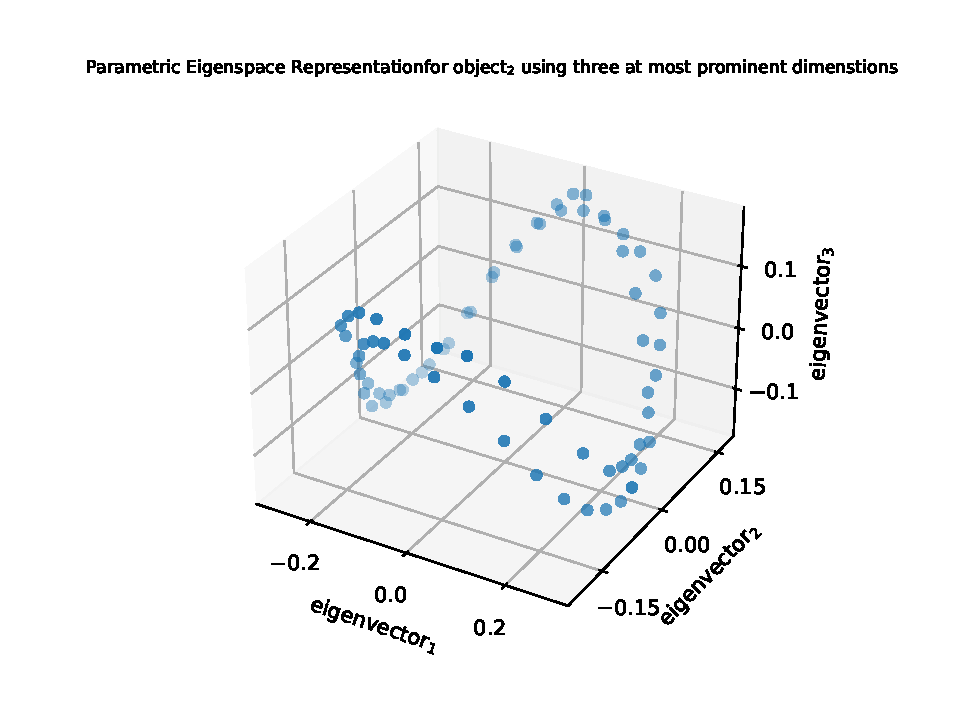
\includegraphics[width = \linewidth]{manifold_scatter_2.pdf}
            \caption{Available Poses of object}
        \end{subfigure}
        \begin{subfigure}{0.45\linewidth}
            \centering
            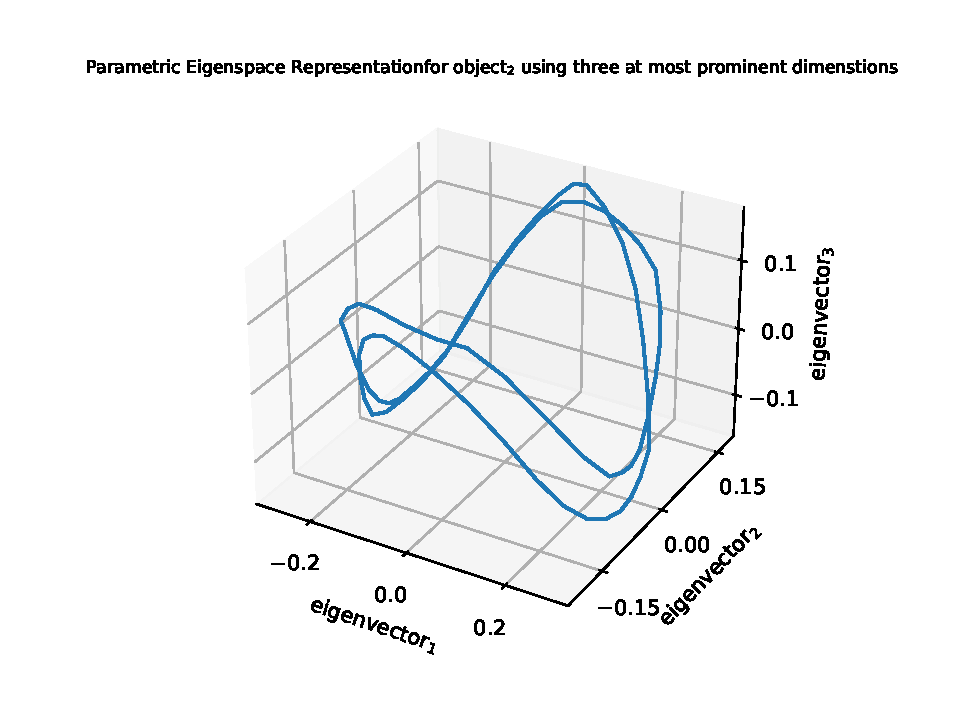
\includegraphics[width = \linewidth]{manifold_plot_2.pdf}
            \caption{Manifold (Cubic Spline interpolation)}
        \end{subfigure}
        \caption{Object 2}
    \end{figure}
\end{itemize}
\end{frame}
\subsection{Dataset}
\begin{frame}{Dataset}{Columbia University Image Library
(COIL-100)}
100 objects! Each object has 72 pose images with pose angle $\{0,5,10,\ldots,345,350,355\}$
    \begin{figure}
        \centering
        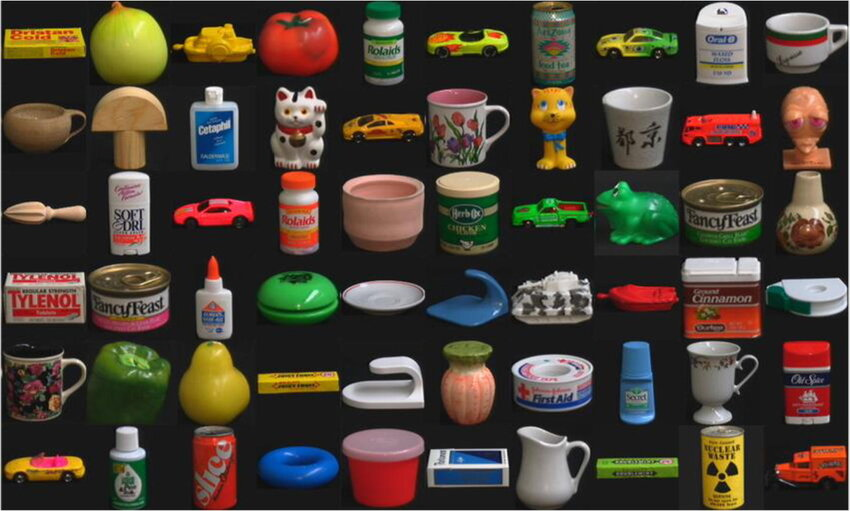
\includegraphics[width=0.45\linewidth]{Sample-images-from-COIL-100-database.jpg}
        \caption{COIL-100 Dataset by Columbia Imaging and Vision Laboratory (CAVE)\footnote{``Columbia Object Image Library,''
S. A. Nene, S. K. Nayar and H. Murase, CUCS-006-96, February 1996.}}
        \label{fig:dataset}
    \end{figure}
\vspace{-1em}
These objects can be categorised into two sets
\begin{itemize}
    \item uniform reflectance but similar shape
    \item complex reflectance and geometric properties
\end{itemize}
\end{frame}

\begin{frame}{Dataset}{Assumptions}
    COIL-100 dataset satisfies these assumptions
    \begin{itemize}
        \item Image Assumptions
        \begin{itemize}
            \item Background region is assigned zero brightness value
            \item Imaging sensor has a linear response (image brightness is proportional to scene radiance)
            \item Object images
            \begin{itemize}
            \item are not occluded by other objects
            \item can be object segmented from the remaining scene
            \item are invariant to image magnification and illumination intensity as segmented image region is
            \begin{description}
            \item[normalized with respect to scale] re-sampled to fit image size
            \item[normalized with respect to brightness] normalised by dividing euclidean norm
        \end{description}
        \end{itemize}
        \end{itemize}
        \item Object Assumptions
        \begin{itemize}
            \item Neither highly specular nor has a high-frequency texture
        \end{itemize}
    \end{itemize}
\end{frame}

\begin{frame}{Manifold (Parametric Appearance Representation)}{Examples}
    \begin{figure}
        \centering
        \begin{subfigure}{0.32\linewidth}
            \centering
            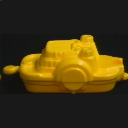
\includegraphics[width = 0.6\linewidth]{splines/obj3__0.png}
            \vspace{1em}
            \caption{Object 2}
        \end{subfigure}
        \begin{subfigure}{0.32\linewidth}
            \centering
            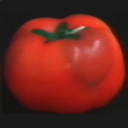
\includegraphics[width = 0.6\linewidth]{splines/obj4__0.png}
            \vspace{1em}
            \caption{Object 3}
        \end{subfigure}
        \begin{subfigure}{0.32\linewidth}
            \centering
            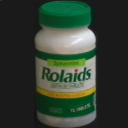
\includegraphics[width = 0.6\linewidth]{splines/obj5__0.png}
            \vspace{1em}
            \caption{Object 4}
        \end{subfigure}
        \begin{subfigure}{0.32\linewidth}
            \centering
            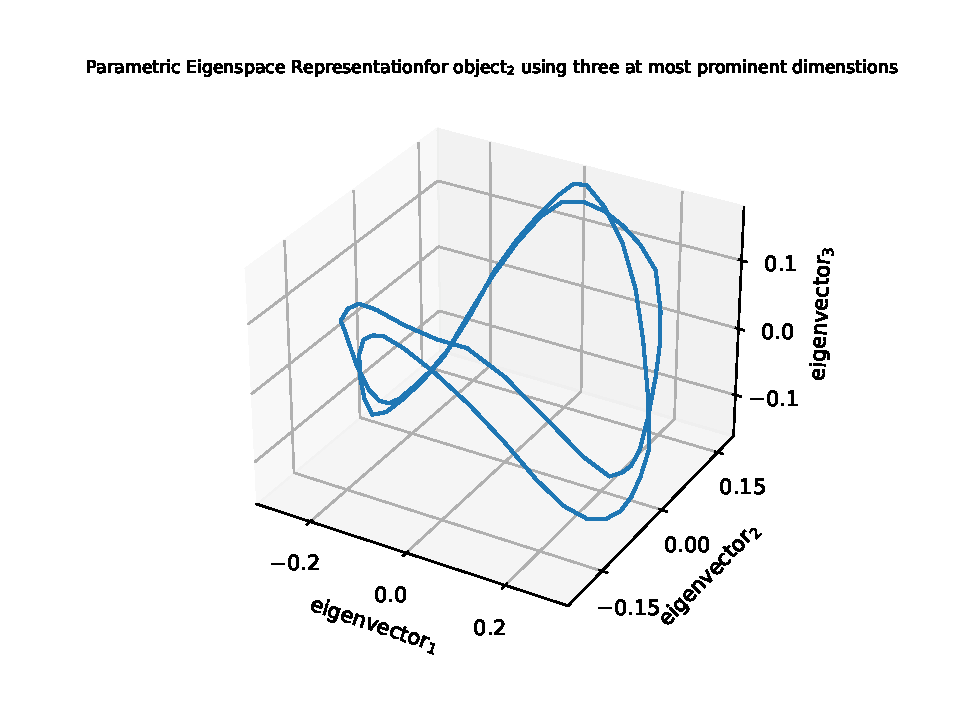
\includegraphics[width = \linewidth]{splines/2.pdf}
            \caption{Corresponding Manifold}
        \end{subfigure}
        \begin{subfigure}{0.32\linewidth}
            \centering
            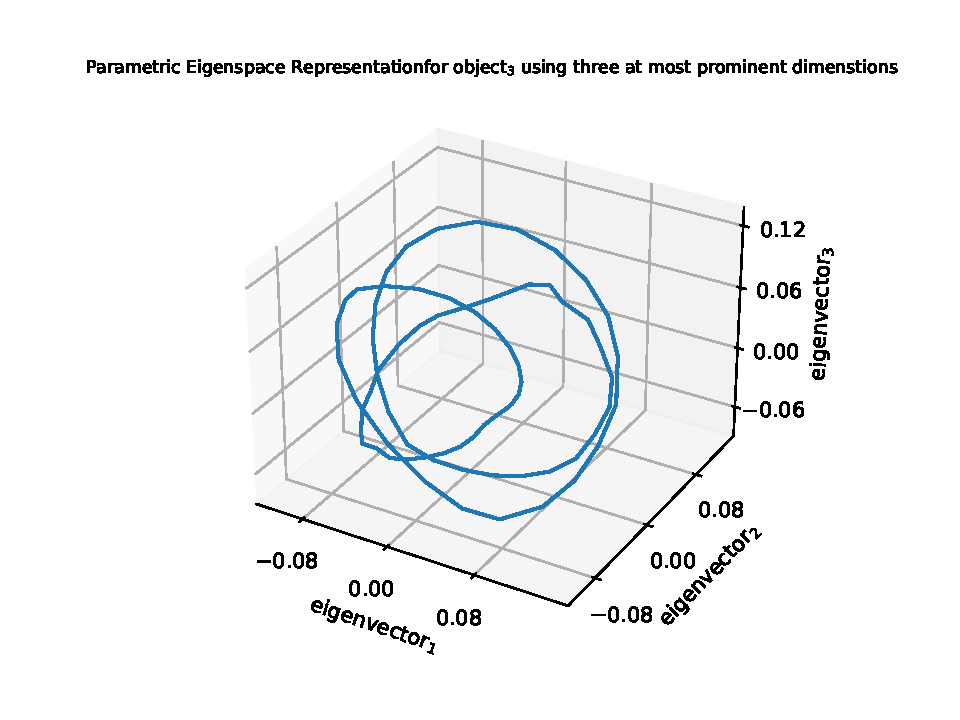
\includegraphics[width = \linewidth]{splines/3.pdf}
            \caption{Corresponding Manifold}
        \end{subfigure}
        \begin{subfigure}{0.32\linewidth}
            \centering
            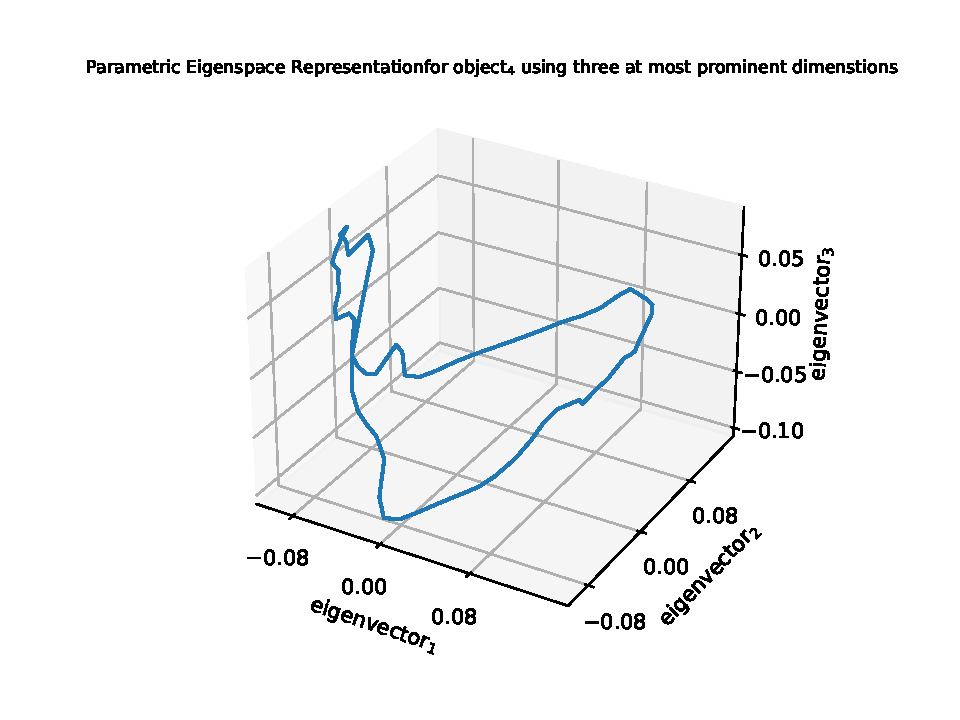
\includegraphics[width = \linewidth]{splines/4.pdf}
            \caption{Corresponding Manifold}
        \end{subfigure}
    \end{figure}
\end{frame}
\subsection{Code Optimizations}
\begin{frame}[fragile]{Code Optimizations}{Implementation}
    \begin{itemize}
        \item Principal Component Analysis (PCA)
        \begin{itemize}
            \item Eigenvector computation of $X^TX$ instead of the covariance matrix ($XX^T$)
            \item \verb!numpy.linalg.eigh! instead to \verb!numpy.linalg.eig! to exploit the algorithms assuming symmetric input matrices
        \end{itemize}
        \item Extensive usage of \verb!numpy! objects and functions to facilitate multi-threading in \verb!numba!
        \item \verb!os.environ[`OMP_NUM_THREADS'] = `16'! to increase number of parallel threads to 16
        \item Ability to store and load saved learnt variables using \verb!pickle!
    \end{itemize}
\end{frame}
\section{Results and Observations}
\subsection{Optimal PCA Threshold and Training Data Split}
\subsection{Variation with PCA Threshold and Training Data Split one at a time}
\begin{frame}{Optimal Values}{PCA Threshold = 0.6 and Training Data Split = 0.7}
    \begin{description}
        \item[Object Recognition accuracy]  99.172\%
        \item[Pose Estimation accuracy] 76.172\%
        \item[Mean Pose error] 6.872$^\circ$
    \end{description}
    In the next two slides, we see some examples of incorrect recognition. 
    
    Even in such cases we see that our model's outputs are reasonable.
    \begin{itemize}
        \item 180$^\circ$ pose errors are most frequent among pose recognition
        \item similar-looking objects get recognised incorrectly
    \end{itemize}
    These errors usually occur in bursts (consecutive poses), which implies that nearby points in manifolds might be too far to interpolate in between points accurately.
    
    One way to solve this is by training on uniformly pose-separated object images.
    
\end{frame}
\subsection{Incorrect Object Detection}
\begin{frame}{Incorrect Object Detection (True and Estimated)}
    \begin{figure}
        \centering
        % \begin{subfigure}{0.32\linewidth}
        %     \centering
        %     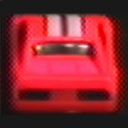
\includegraphics[width = 0.6\linewidth]{incorrect/obj23__90.png}
        %     \vspace{1em}
        %     \caption{Obect 22, Angle 90}
        % \end{subfigure}
        \begin{subfigure}{0.32\linewidth}
            \centering
            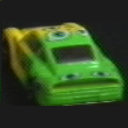
\includegraphics[width = 0.6\linewidth]{incorrect/obj8__75.png}
            \vspace{1em}
            \caption{Obect 7, Angle 75}
        \end{subfigure}
        \begin{subfigure}{0.32\linewidth}
            \centering
            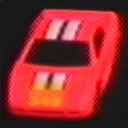
\includegraphics[width = 0.6\linewidth]{incorrect/obj23__280.png}
            \vspace{1em}
            \caption{Obect 22, Angle 280}
        \end{subfigure}
        \begin{subfigure}{0.32\linewidth}
            \centering
            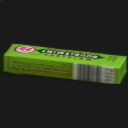
\includegraphics[width = 0.6\linewidth]{incorrect/obj98__195.png}
            \vspace{1em}
            \caption{Obect 97, Angle 195}
        \end{subfigure}
        % \begin{subfigure}{0.32\linewidth}
        %     \centering
        %     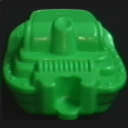
\includegraphics[width = 0.6\linewidth]{incorrect/obj78__90.png}
        %     \vspace{1em}
        %     \caption{Object 77, Angle 90}
        % \end{subfigure}
        \begin{subfigure}{0.32\linewidth}
            \centering
            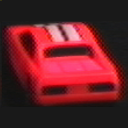
\includegraphics[width = 0.6\linewidth]{incorrect/obj23__80.png}
            \vspace{1em}
            \caption{Object 22, Angle 80}
        \end{subfigure}
        \begin{subfigure}{0.32\linewidth}
            \centering
            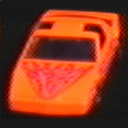
\includegraphics[width = 0.6\linewidth]{incorrect/obj76__280.png}
            \vspace{1em}
            \caption{Object 75, Angle 280}
        \end{subfigure}
        \begin{subfigure}{0.32\linewidth}
            \centering
            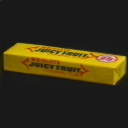
\includegraphics[width = 0.6\linewidth]{incorrect/obj84__25.png}
            \vspace{1em}
            \caption{Object 83, Angle 25}
        \end{subfigure}
    \end{figure}
\end{frame}
\begin{frame}{Incorrect Pose Recognition (True and Estimated)}
    \begin{figure}
        \centering
        \begin{subfigure}{0.32\linewidth}
            \centering
            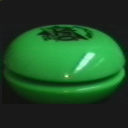
\includegraphics[width = 0.6\linewidth]{incorrect/obj34__75.png}
            \vspace{1em}
            \caption{Obect 33, Angle 75}
        \end{subfigure}
        \begin{subfigure}{0.32\linewidth}
            \centering
            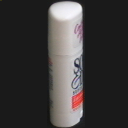
\includegraphics[width = 0.6\linewidth]{incorrect/obj22__280.png}
            \vspace{1em}
            \caption{Obect 21, Angle 280}
        \end{subfigure}
        \begin{subfigure}{0.32\linewidth}
            \centering
            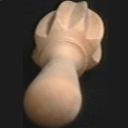
\includegraphics[width = 0.6\linewidth]{incorrect/obj21__100.png}
            \vspace{1em}
            \caption{Obect 20, Angle 100}
        \end{subfigure}
        \begin{subfigure}{0.32\linewidth}
            \centering
            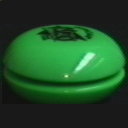
\includegraphics[width = 0.6\linewidth]{incorrect/obj34__80.png}
            \vspace{1em}
            \caption{Object 33, Angle 80}
        \end{subfigure}
        \begin{subfigure}{0.32\linewidth}
            \centering
            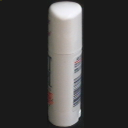
\includegraphics[width = 0.6\linewidth]{incorrect/obj22__95.png}
            \vspace{1em}
            \caption{Object 21, Angle 95}
        \end{subfigure}
        \begin{subfigure}{0.32\linewidth}
            \centering
            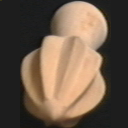
\includegraphics[width = 0.6\linewidth]{incorrect/obj21__280.png}
            \vspace{1em}
            \caption{Object 20, Angle 280}
        \end{subfigure}
    \end{figure}
\end{frame}
\begin{frame}{Variation with PCA Threshold and Training Data Split one at a time}
    In the coming plots, we vary each parameter one by one and then vary them simultaneously
    \begin{itemize}
        \item Vary PCA Threshold as $\{0.05, 0.1,\ldots, 0.9, 0.95\}$, set Training Data Split to 0.6
        \begin{itemize}
            \item higher PCA Threshold leads to overfitting 
        \end{itemize}
        \item Vary Training Data Split as $\{0.05, 0.1,\ldots, 0.9, 0.95\}$, set PCA Threshold to 0.7
        \begin{itemize}
            \item more training data creates more accurate manifold which leads to better recognition
        \end{itemize}
        \item Vary PCA Threshold as $\{0.05, 0.1,\ldots, 0.9, 0.95\}$ and 
        
        vary Training Data Split as $\{0.05, 0.1,\ldots, 0.9, 0.95\}$
    \end{itemize}
\end{frame}
\begin{frame}{Variation with PCA Threshold and Training Data Split one at a time}{Accuracy}
    \begin{figure}
        \centering
        \begin{subfigure}{0.48\linewidth}
            \centering
            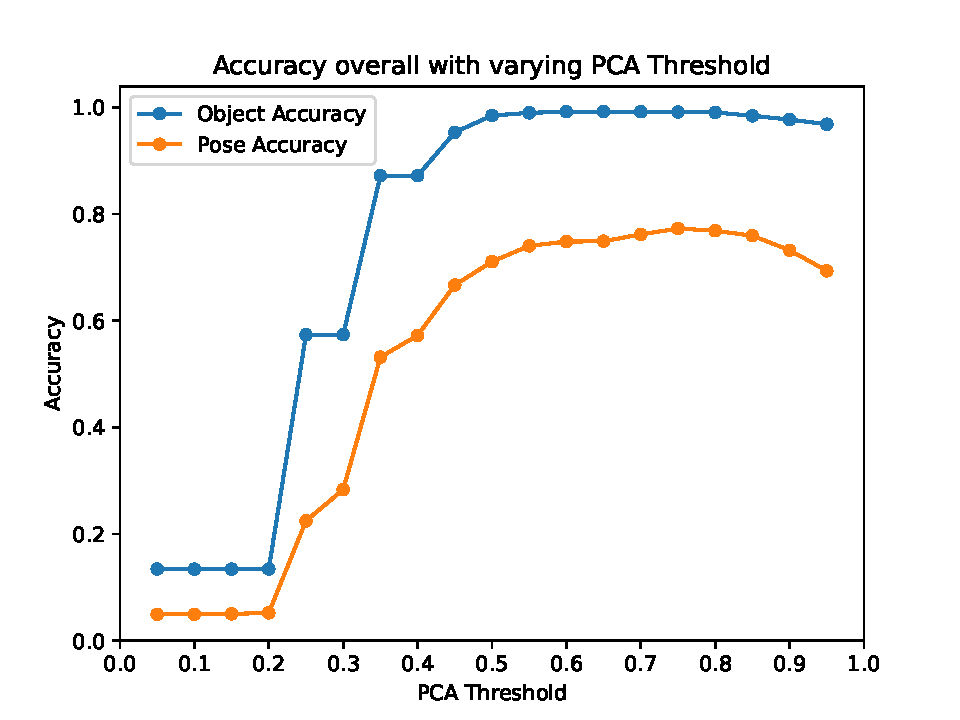
\includegraphics[width=\linewidth]{pca/accuracy_overall.pdf}
        \end{subfigure}
        \begin{subfigure}{0.48\linewidth}
            \centering
            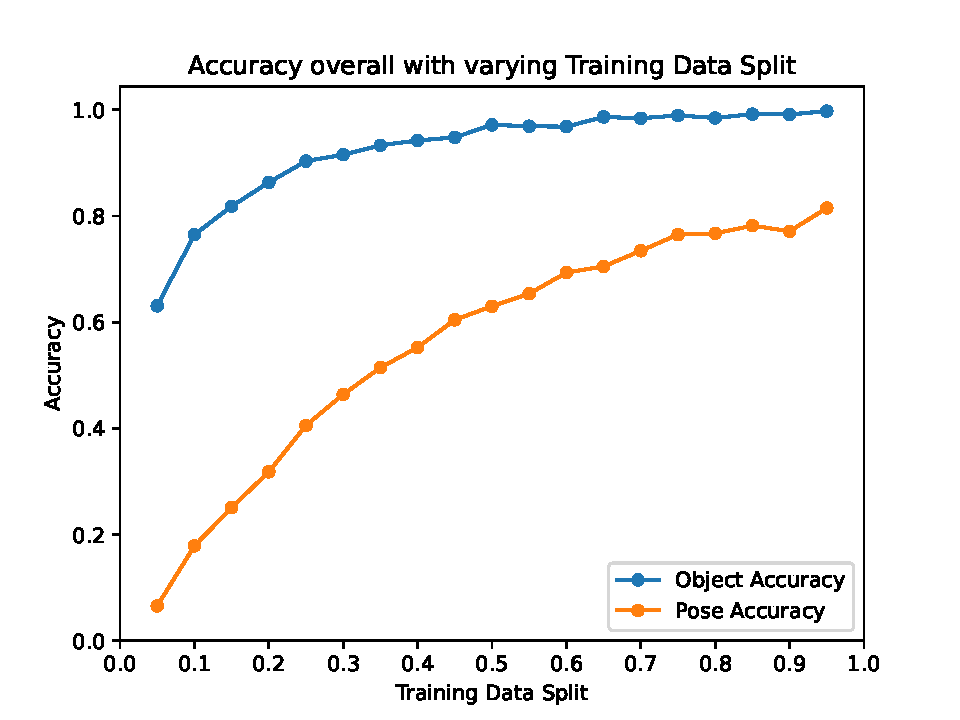
\includegraphics[width=\linewidth]{tds/accuracy_overall.pdf}
        \end{subfigure}
    \end{figure}
\end{frame}
\begin{frame}{Variation with PCA Threshold and Training Data Split one at a time}{Mean Error}
    \begin{figure}
        \centering
        \begin{subfigure}{0.48\linewidth}
            \centering
            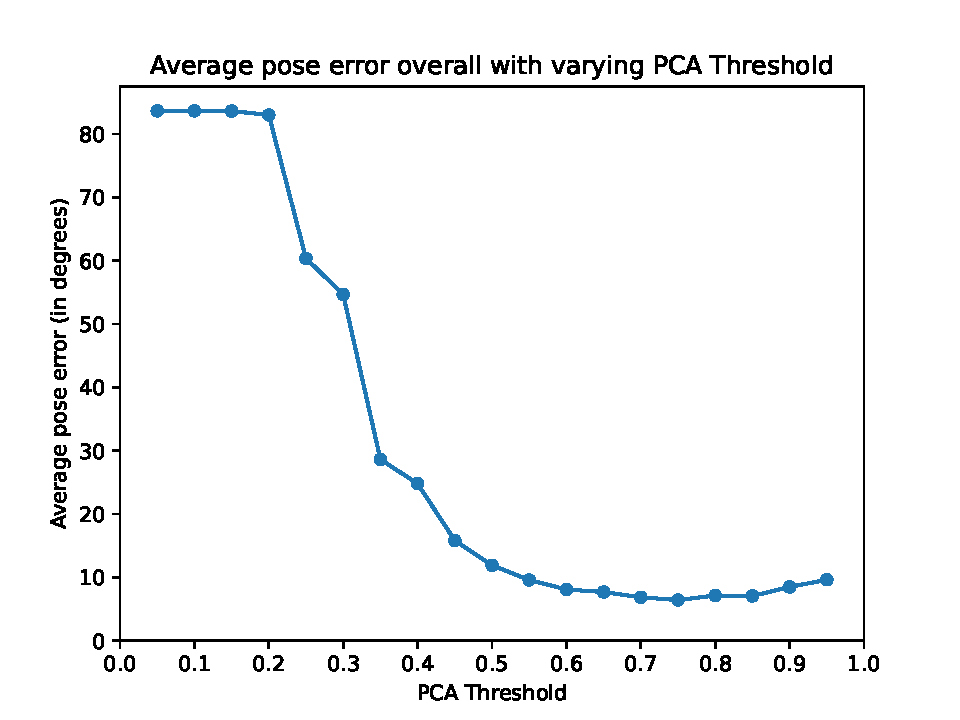
\includegraphics[width=\linewidth]{pca/mean_error_overall.pdf}
        \end{subfigure}
        \begin{subfigure}{0.48\linewidth}
            \centering
            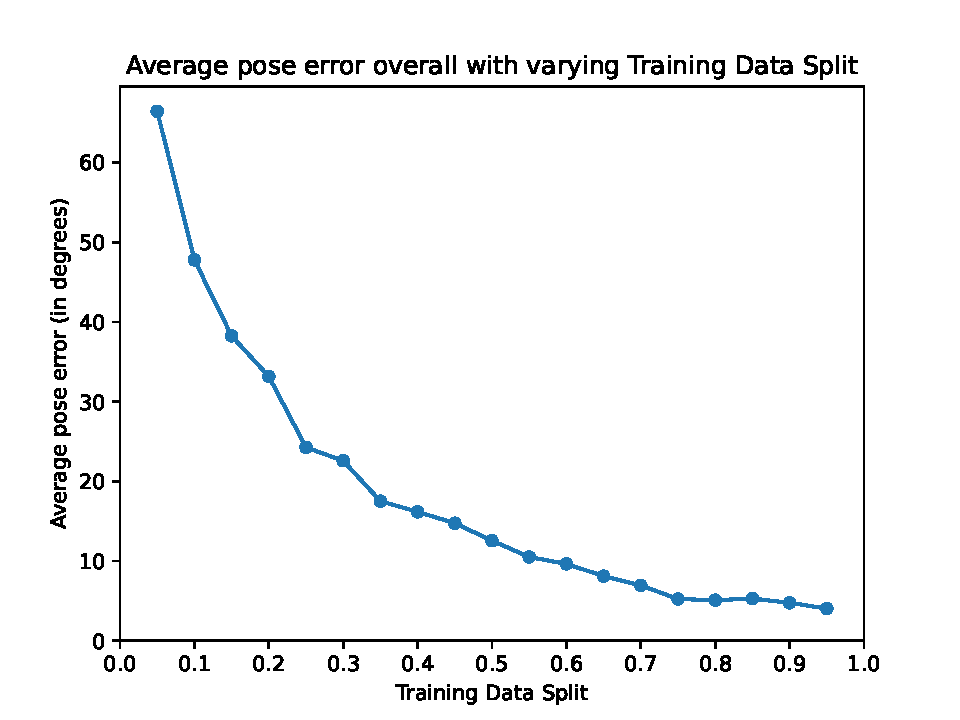
\includegraphics[width=\linewidth]{tds/mean_error_overall.pdf}
        \end{subfigure}
    \end{figure}
\end{frame}
\begin{frame}{Variation with PCA Threshold and Training Data Split one at a time}{Object Accuracy}
    \begin{figure}
        \centering
        \begin{subfigure}{0.48\linewidth}
            \centering
            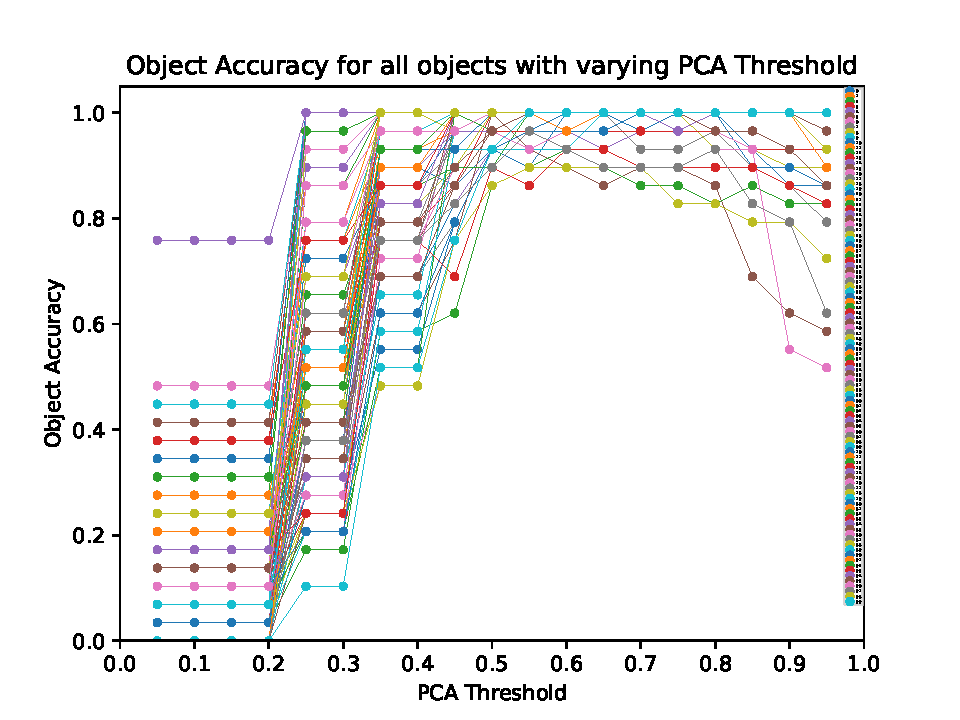
\includegraphics[width=\linewidth]{pca/object_accuracy_all_objects.pdf}
        \end{subfigure}
        \begin{subfigure}{0.48\linewidth}
            \centering
            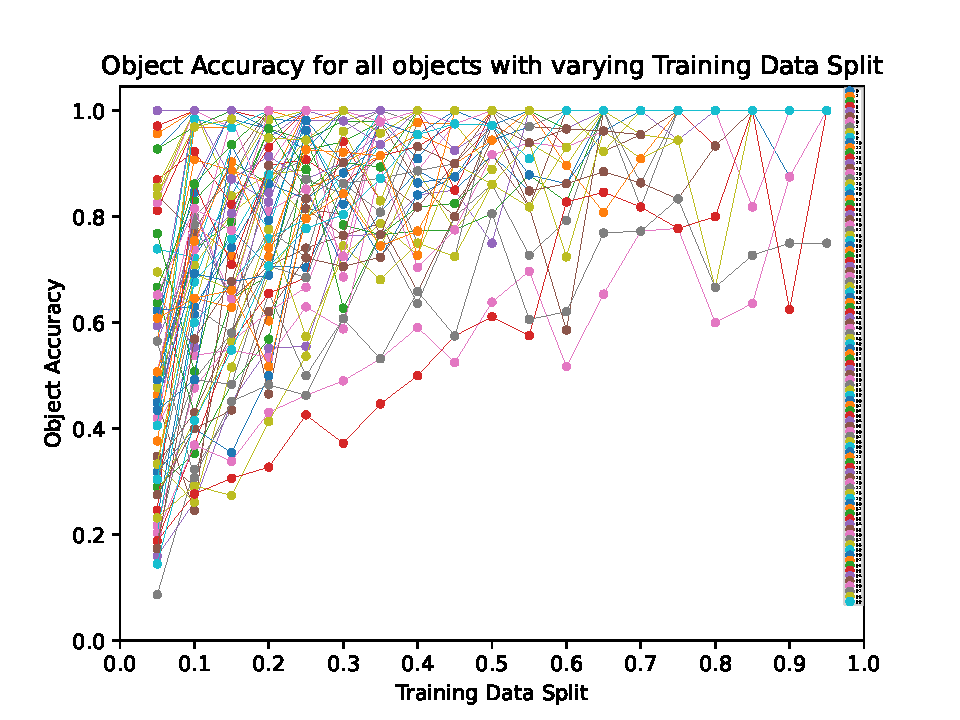
\includegraphics[width=\linewidth]{tds/object_accuracy_all_objects.pdf}
        \end{subfigure}
    \end{figure}
\end{frame}
\begin{frame}{Variation with PCA Threshold and Training Data Split one at a time}{Pose Accuracy}
    \begin{figure}
        \centering
        \begin{subfigure}{0.48\linewidth}
            \centering
            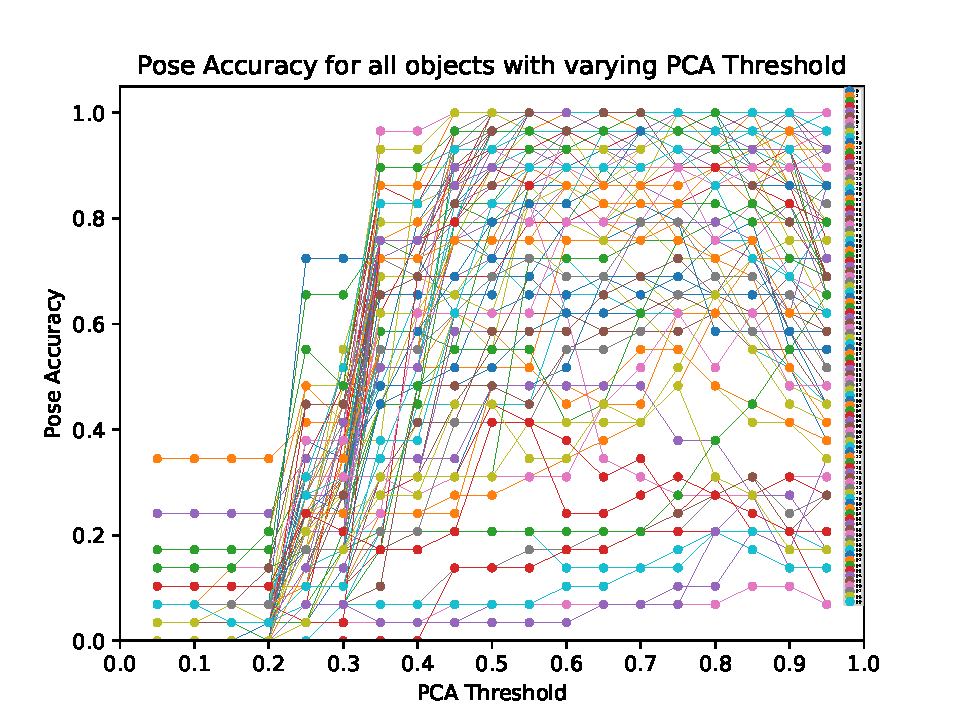
\includegraphics[width=\linewidth]{pca/pose_accuracy_all_objects.pdf}
        \end{subfigure}
        \begin{subfigure}{0.48\linewidth}
            \centering
            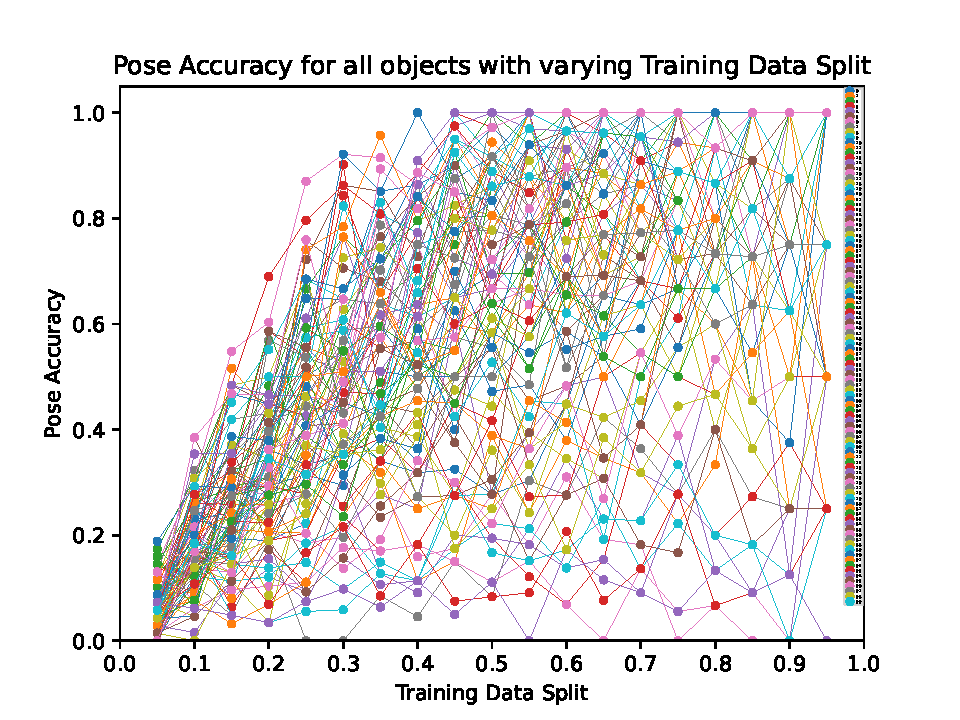
\includegraphics[width=\linewidth]{tds/pose_accuracy_all_objects.pdf}
        \end{subfigure}
    \end{figure}
\end{frame}
\begin{frame}{Variation with PCA Threshold and Training Data Split one at a time}{Mean Error}
    \begin{figure}
        \centering
        \begin{subfigure}{0.48\linewidth}
            \centering
            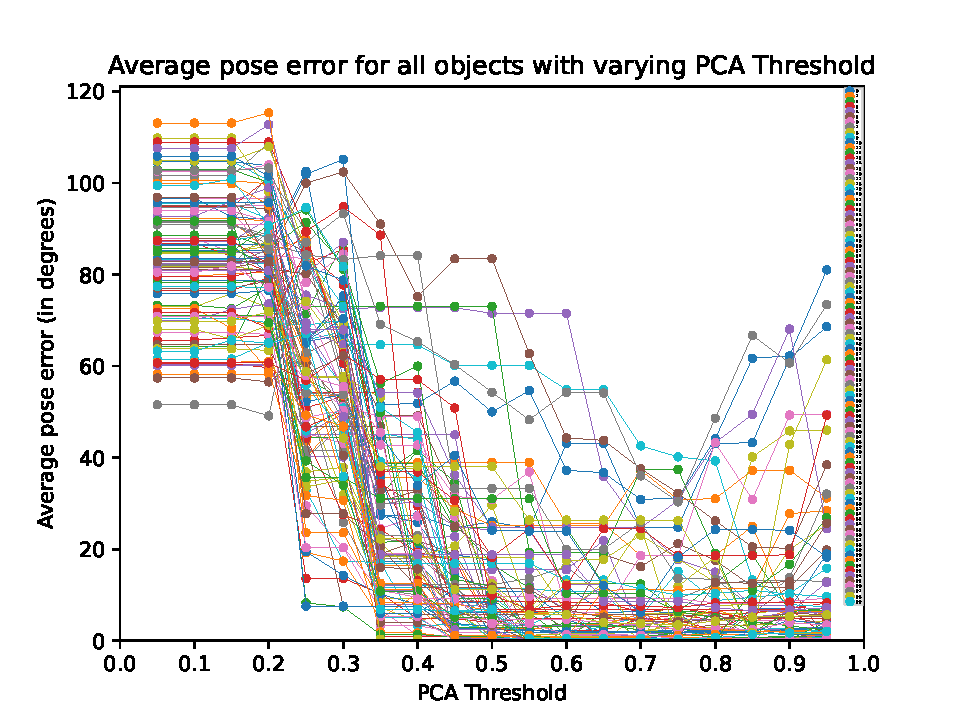
\includegraphics[width=\linewidth]{pca/mean_error_all_objects.pdf}
        \end{subfigure}
        \begin{subfigure}{0.48\linewidth}
            \centering
            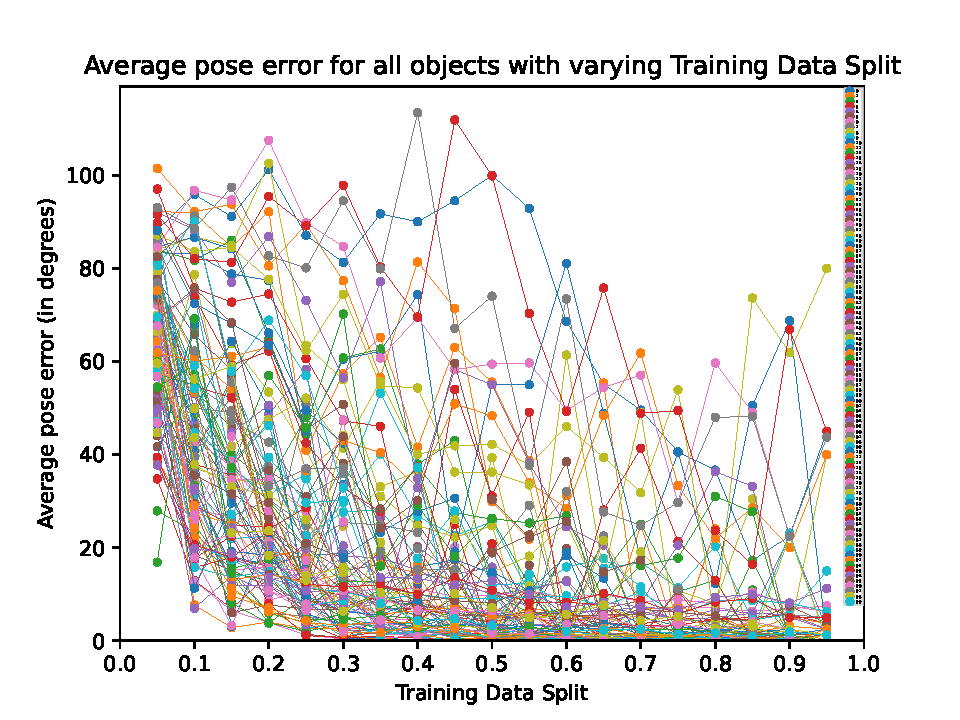
\includegraphics[width=\linewidth]{tds/mean_error_all_objects.pdf}
        \end{subfigure}
    \end{figure}
\end{frame}
\begin{frame}{Variation with PCA Threshold and Training Data Split one at a time}{Exact Error}
    \begin{figure}
        \centering
        \begin{subfigure}{0.48\linewidth}
            \centering
            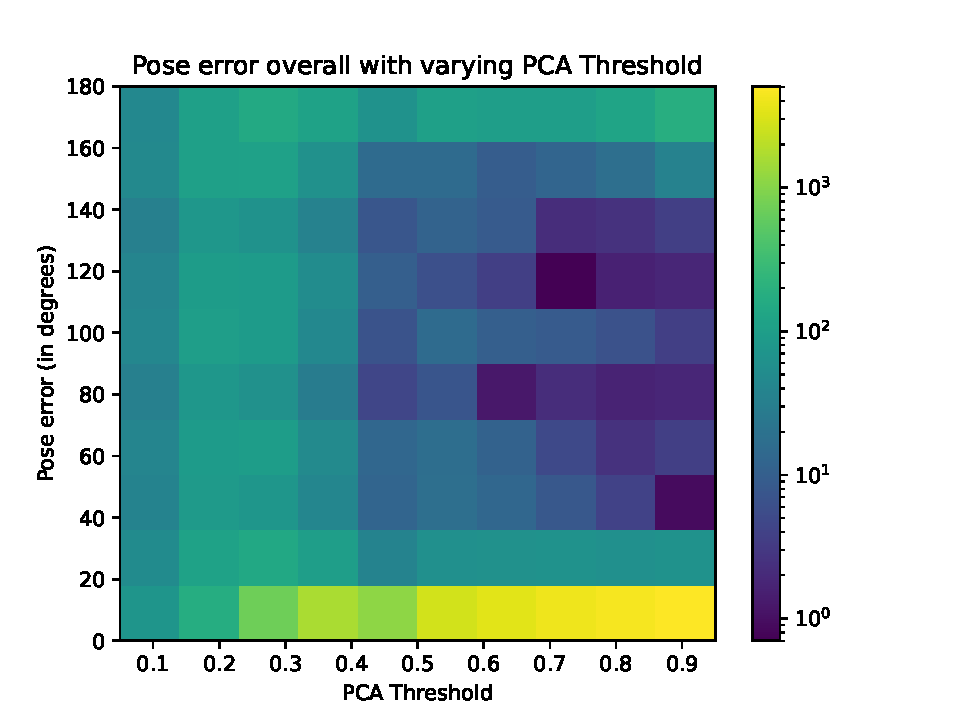
\includegraphics[width=\linewidth]{pca/error_histogram_overall.pdf}
        \end{subfigure}
        \begin{subfigure}{0.48\linewidth}
            \centering
            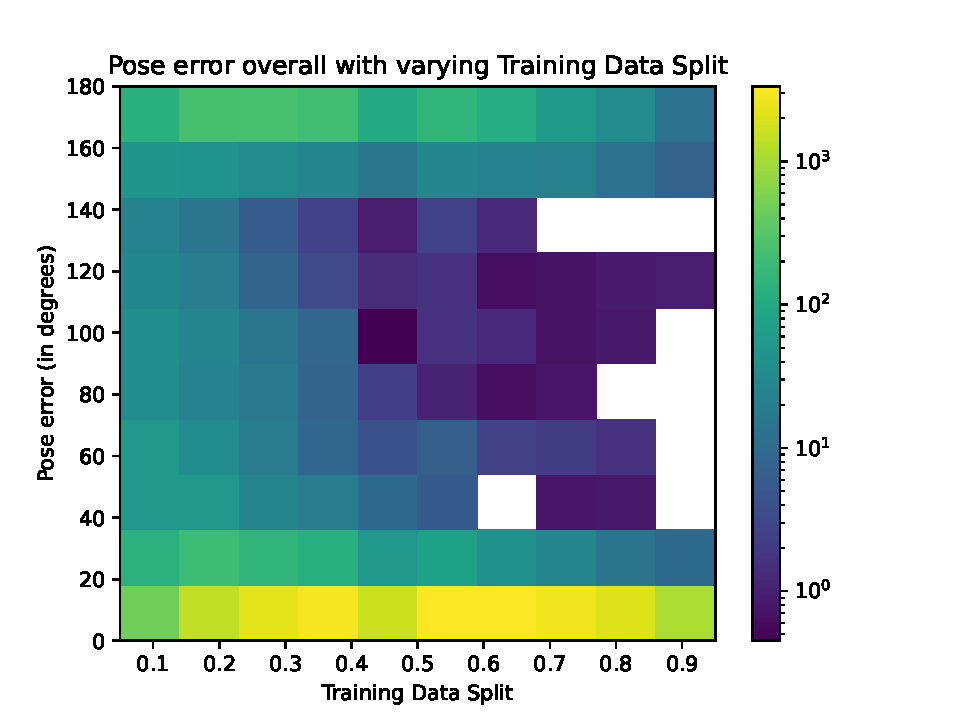
\includegraphics[width=\linewidth]{tds/error_histogram_overall.pdf}
        \end{subfigure}
    \end{figure}
\end{frame}
\subsection{Simultaneous variation with PCA Threshold and Training Data Split}
\begin{frame}{Simultaneous variation with PCA Threshold and Training Data Split}
    \begin{figure}
        \centering
        \begin{subfigure}{0.32\linewidth}
            \centering
            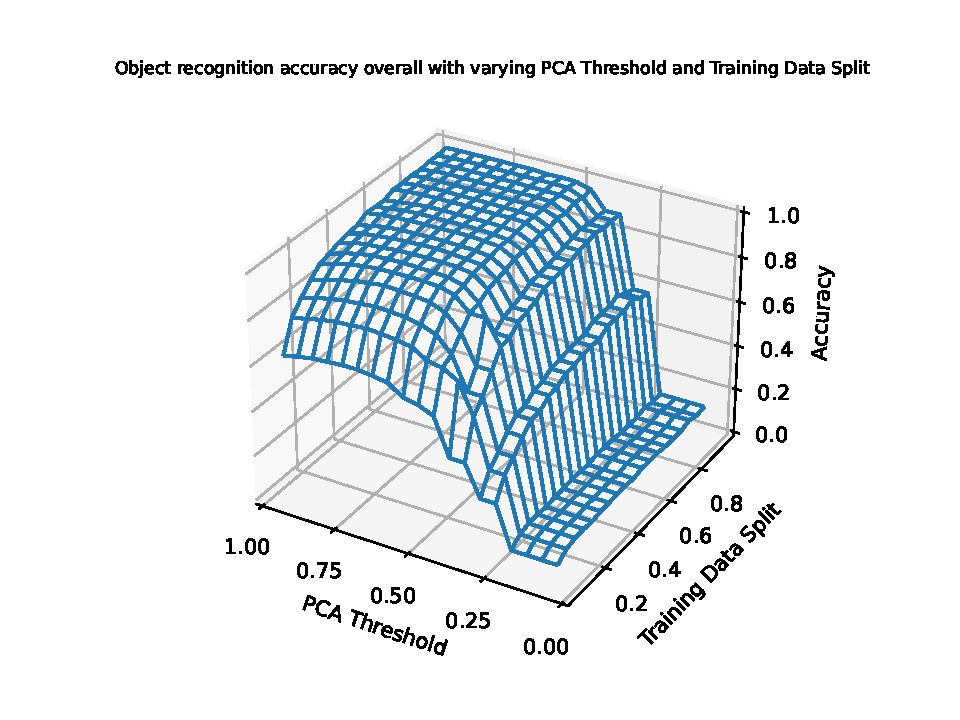
\includegraphics[width=\linewidth]{combined/object_accuracy_overall.pdf}
            \caption{Object Accuracy}
        \end{subfigure}
        \begin{subfigure}{0.32\linewidth}
            \centering
            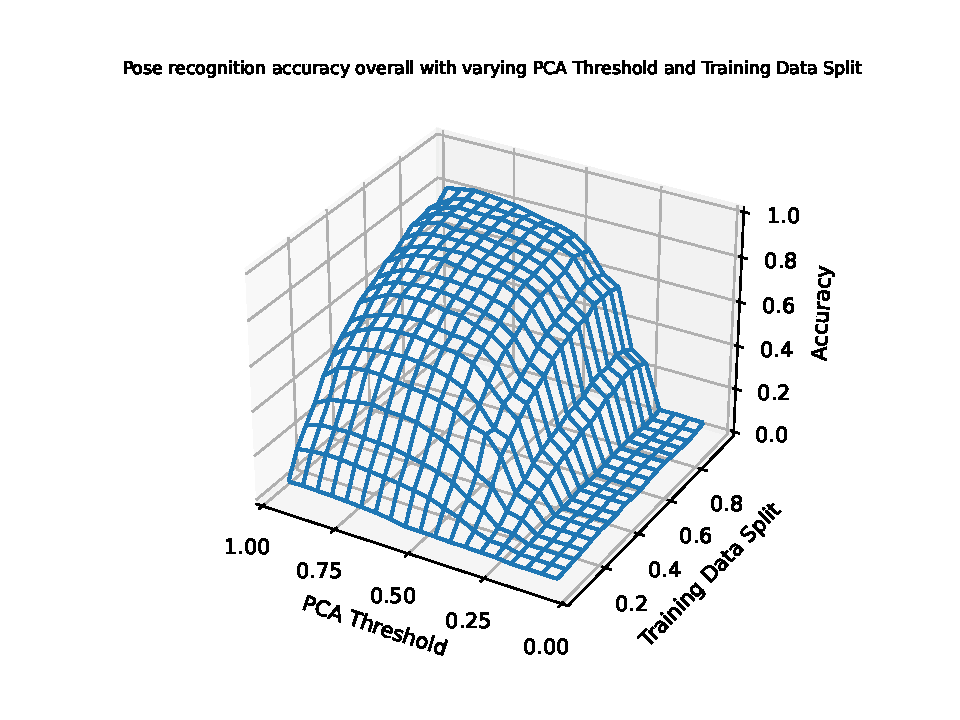
\includegraphics[width=\linewidth]{combined/pose_accuracy_overall.pdf}
            \caption{Pose Accuracy}
        \end{subfigure}
        \begin{subfigure}{0.32\linewidth}
            \centering
            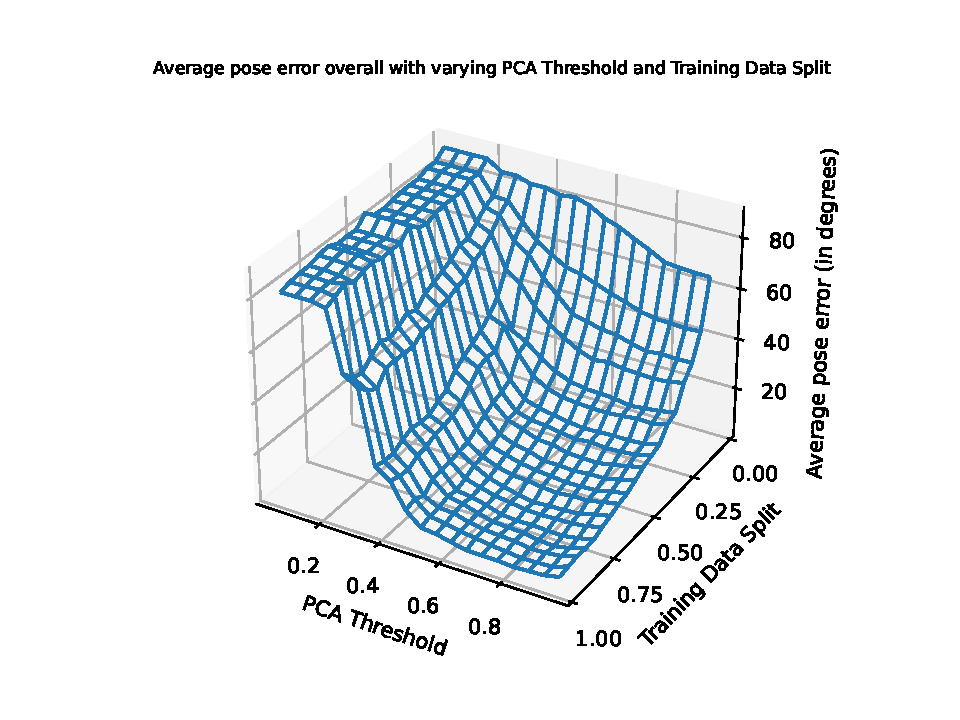
\includegraphics[width=\linewidth]{combined/mean_error_overall.pdf}
            \caption{Mean Error}
        \end{subfigure}
    \end{figure}
\end{frame}
\subsection{Observations (Three types of objects)}
\begin{frame}{Observations}{Three types of objects}
% \begin{enumerate}[(a)]
\begin{itemize}
    \item Simple Objects, almost no variation in poses due to symmetrical nature and less details
    \item Simple Objects, almost no variation in poses due to symmetrical nature but highly detailed
    \item Complex Objects, different shapes in different poses
\end{itemize}
% \end{enumerate}
    \begin{figure}
        \centering
        \begin{subfigure}{0.32\linewidth}
            \centering
            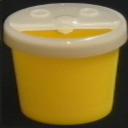
\includegraphics[width = 0.6\linewidth]{wireframe/obj70__0.png}
            \vspace{1em}
            \caption{Object 69}
        \end{subfigure}
        \begin{subfigure}{0.32\linewidth}
            \centering
            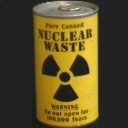
\includegraphics[width = 0.6\linewidth]{wireframe/obj99__0.png}
            \vspace{1em}
            \caption{Object 98}
        \end{subfigure}
        \begin{subfigure}{0.32\linewidth}
            \centering
            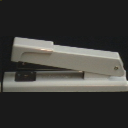
\includegraphics[width = 0.6\linewidth]{wireframe/obj68__0.png}
            \vspace{1em}
            \caption{Object 67}
        \end{subfigure}
    \end{figure}
\end{frame}
\begin{frame}{Observations}{Types of Wireframe: Mean Accuracy}
\begin{itemize}
    \item as object complexity increases, more training data is needed for lower mean error
    \item only slightly higher pca threshold needed for complex objects
\end{itemize}
    \begin{figure}
        \centering
        \begin{subfigure}{0.32\linewidth}
            \centering
            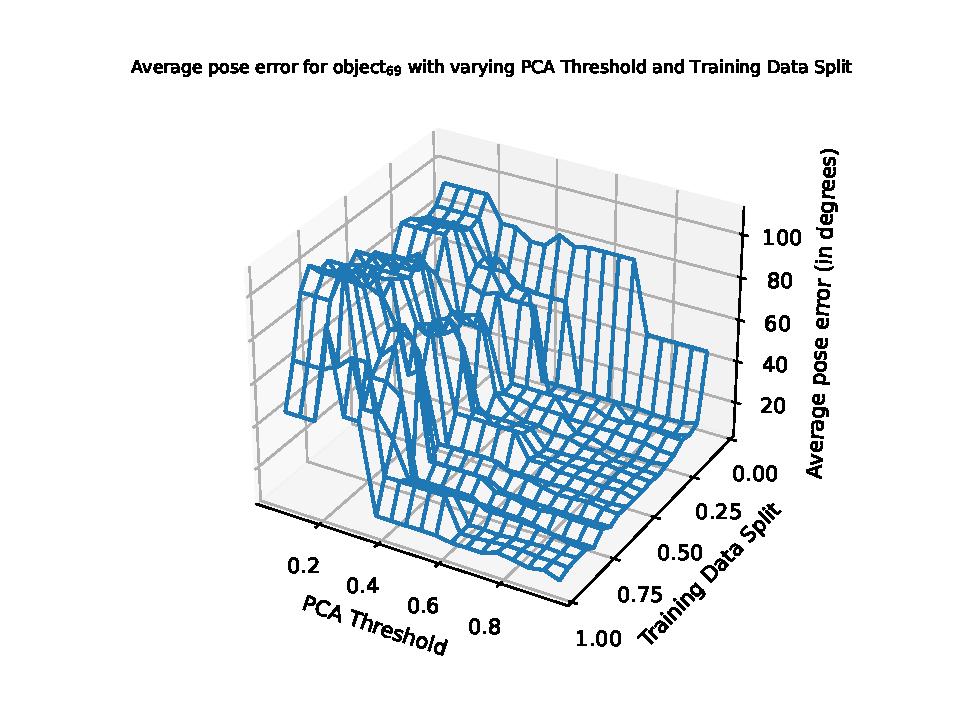
\includegraphics[width=1.2\linewidth]{wireframe/error/69.pdf}
            \caption{Object 69}
        \end{subfigure}
        \begin{subfigure}{0.32\linewidth}
            \centering
            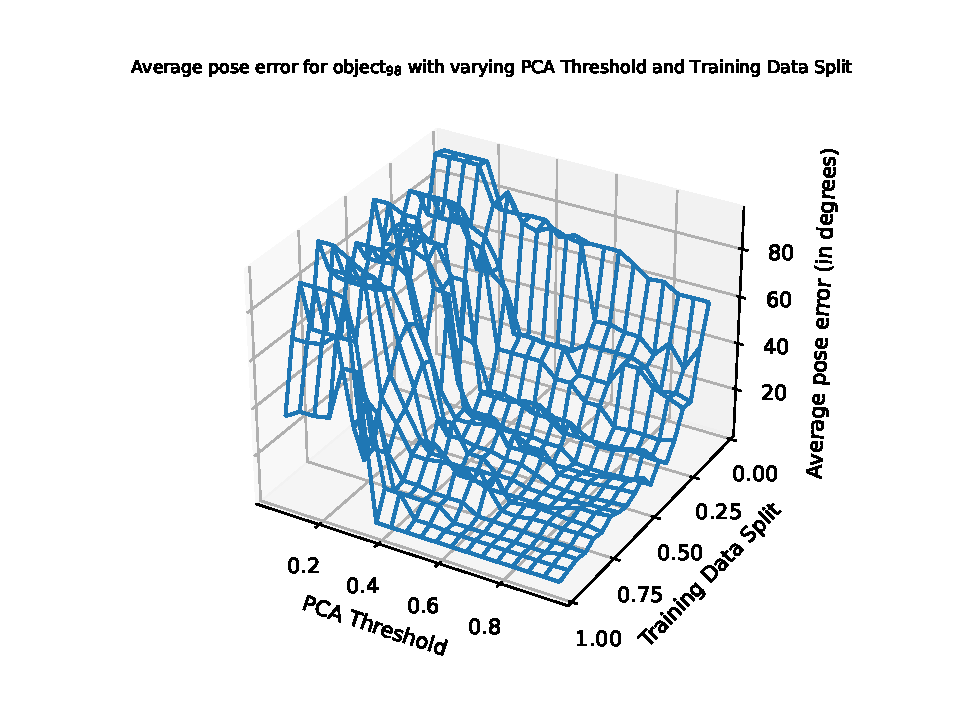
\includegraphics[width=1.2\linewidth]{wireframe/error/98.pdf}
            \caption{Object 98}
        \end{subfigure}
        \begin{subfigure}{0.32\linewidth}
            \centering
            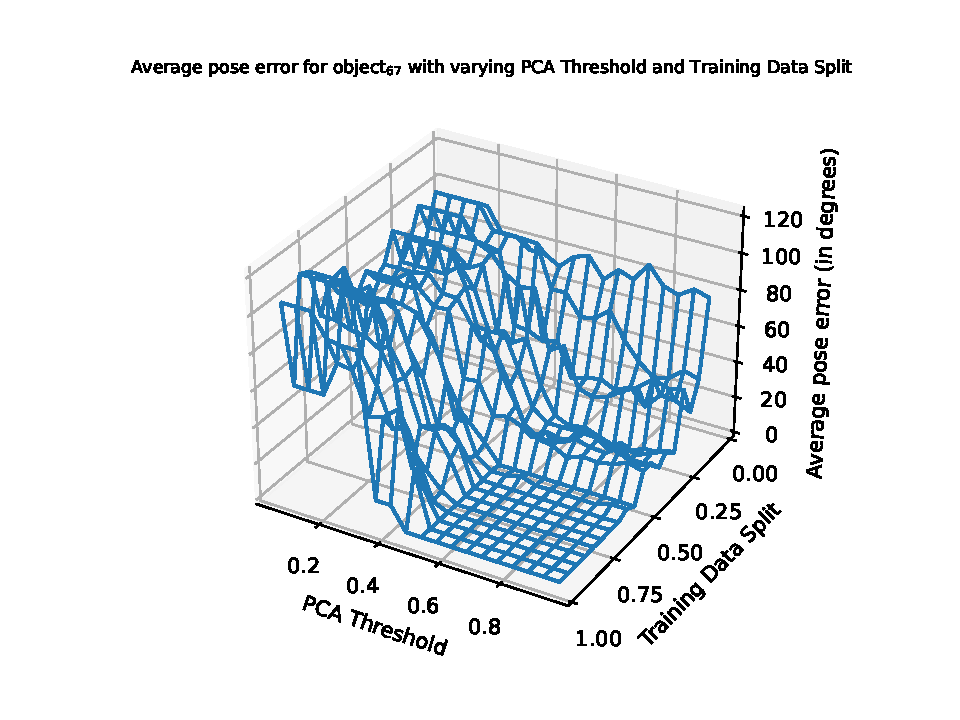
\includegraphics[width=1.2\linewidth]{wireframe/error/67.pdf}
            \caption{Object 67}
        \end{subfigure}
        
    \end{figure}
\end{frame}
\begin{frame}{Observations}{Types of Wireframe: Object Accuracy}
\begin{itemize}
    \item as object complexity increases, more training data is needed for higher accuracy

    15-20 objects poses are enough for learning the simple objects, but 30-40 object poses are needed to learn complex dataset
    \item higher pca threshold only needed in complex objects
\end{itemize}
    \begin{figure}
        \centering
        \begin{subfigure}{0.32\linewidth}
            \centering
            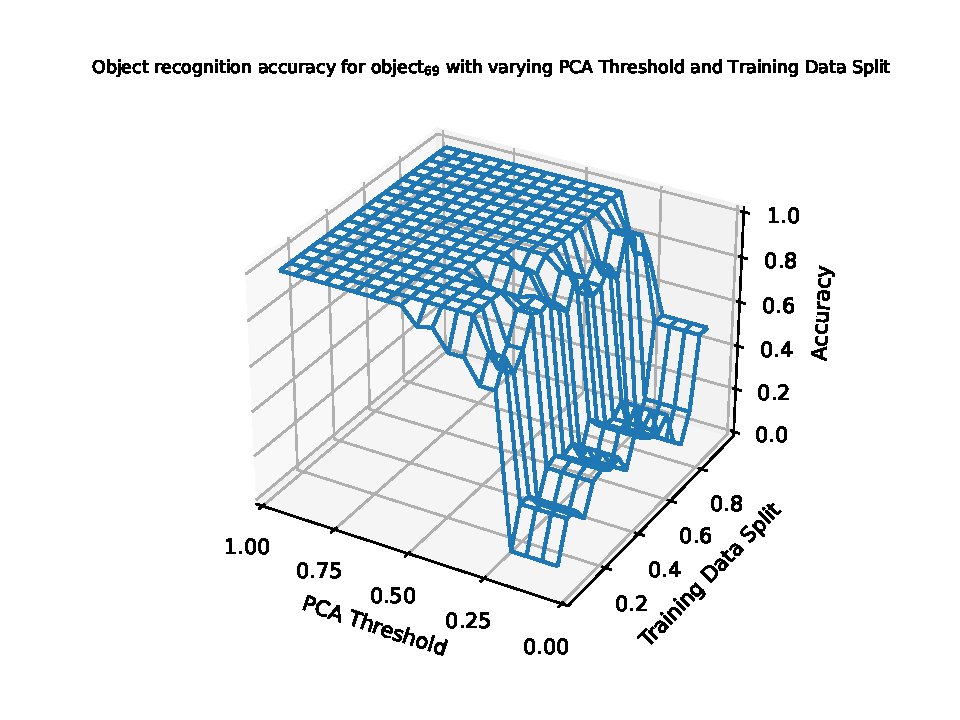
\includegraphics[width=1.2\linewidth]{wireframe/object/69.pdf}
            \caption{Object 69}
        \end{subfigure}
        \begin{subfigure}{0.32\linewidth}
            \centering
            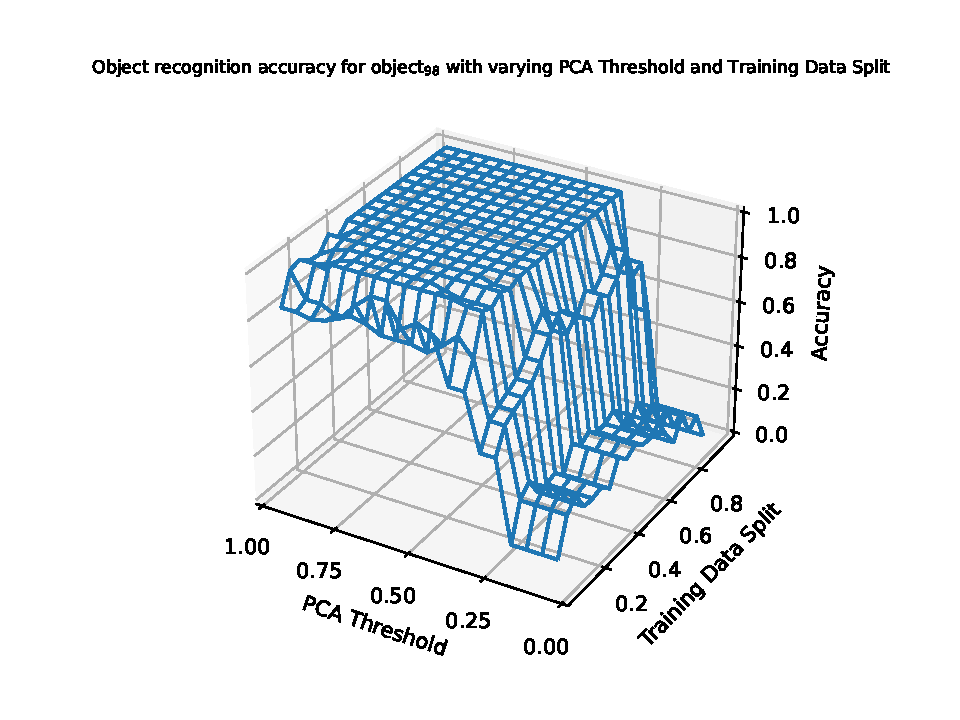
\includegraphics[width=1.2\linewidth]{wireframe/object/98.pdf}
            \caption{Object 98}
        \end{subfigure}
        \begin{subfigure}{0.32\linewidth}
            \centering
            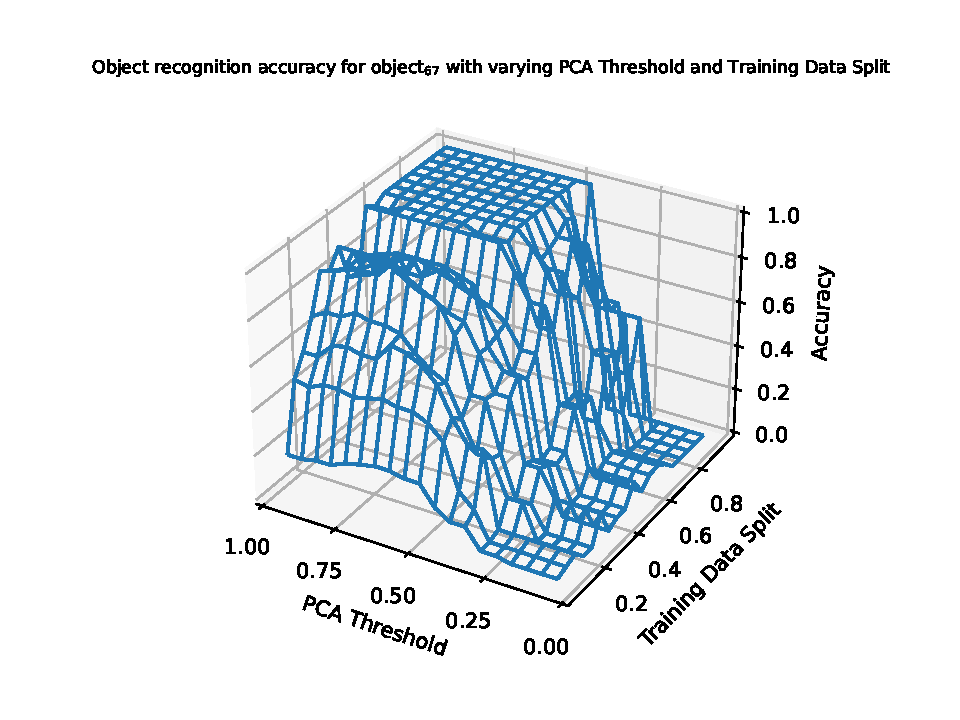
\includegraphics[width=1.2\linewidth]{wireframe/object/67.pdf}
            \caption{Object 67}
        \end{subfigure}
    \end{figure}
\end{frame}
\begin{frame}{Observations}{Types of Wireframe: Pose Accuracy}
\begin{itemize}
    \item accuracy increases as object complexity increases, because pose becomes easier to distinguish
    \item for simpler objects, more training data or pca threshold doesn't help much to estimate exactly
\end{itemize}
    \begin{figure}
        \centering
        \begin{subfigure}{0.32\linewidth}
            \centering
            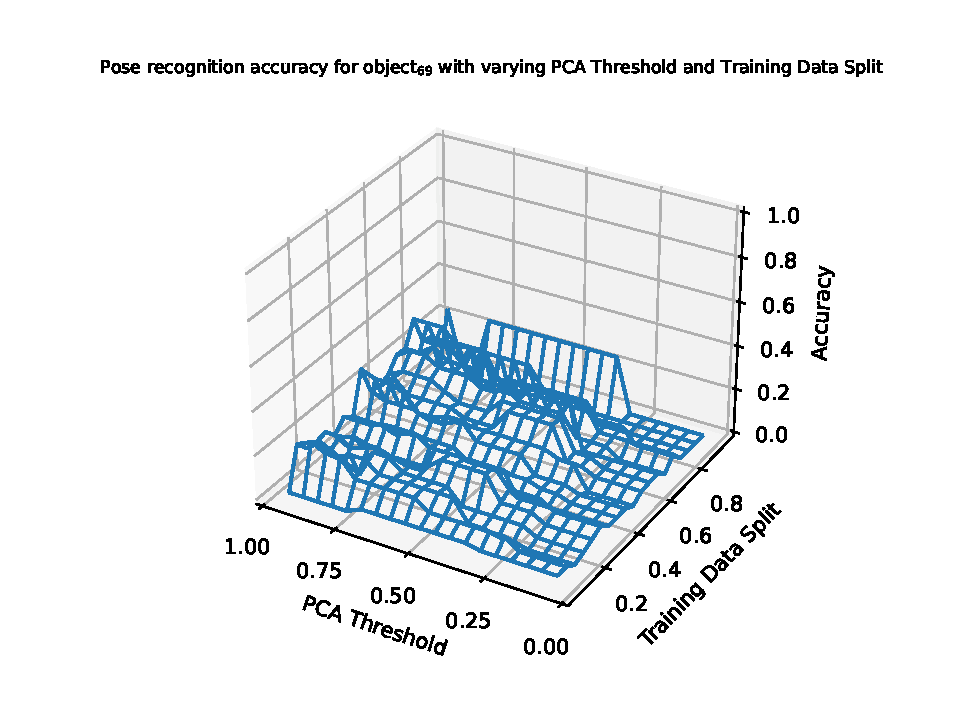
\includegraphics[width=1.2\linewidth]{wireframe/pose/69.pdf}
            \caption{Object 69}
        \end{subfigure}
        \begin{subfigure}{0.32\linewidth}
            \centering
            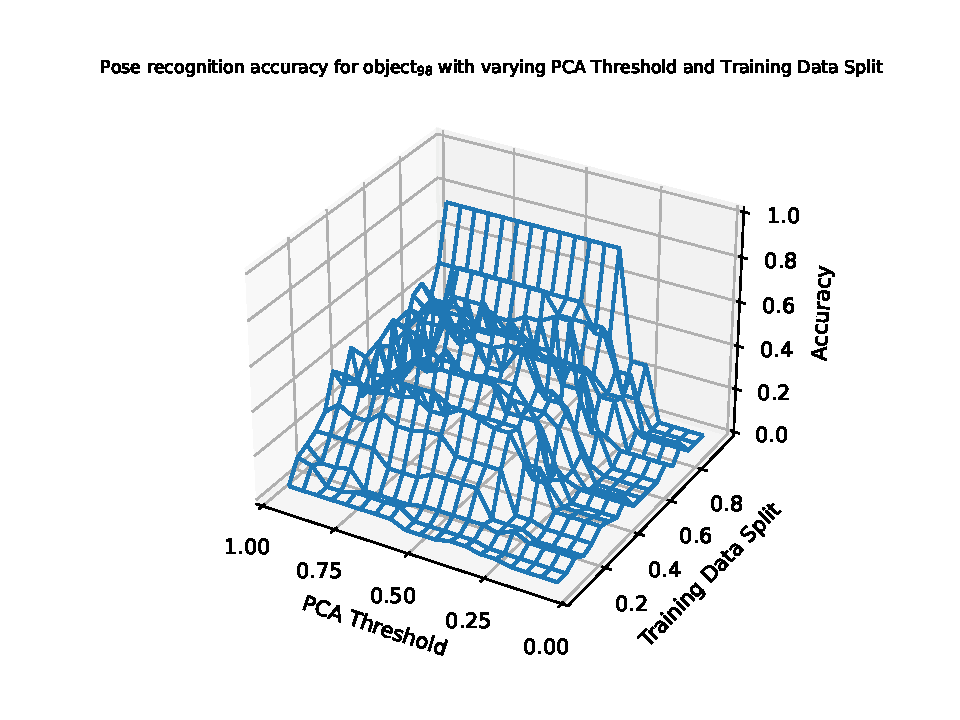
\includegraphics[width=1.2\linewidth]{wireframe/pose/98.pdf}
            \caption{Object 98}
        \end{subfigure}
        \begin{subfigure}{0.32\linewidth}
            \centering
            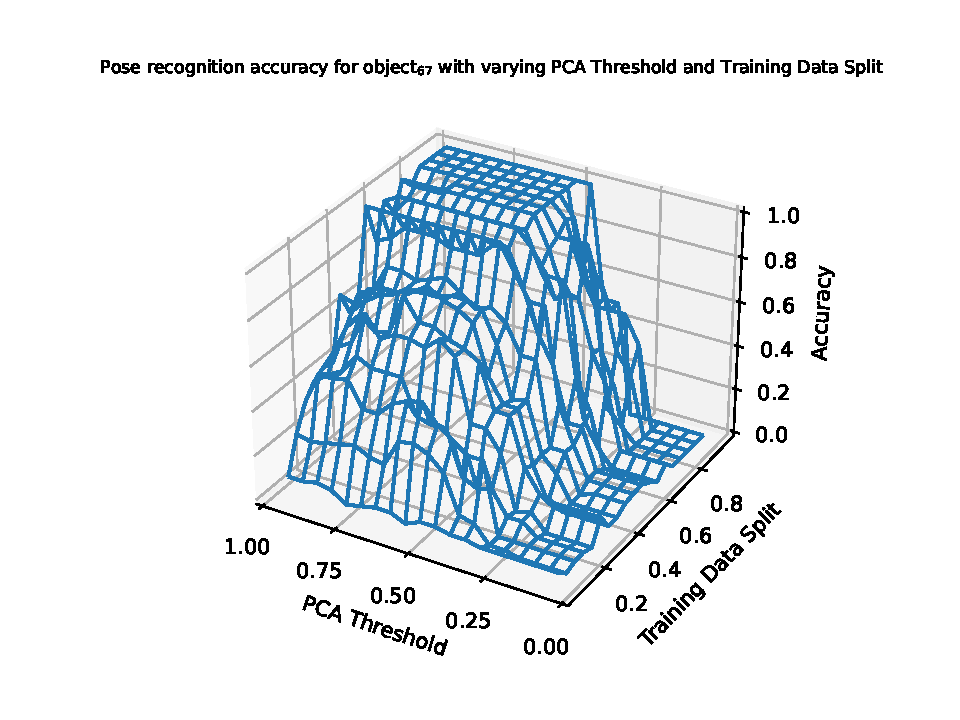
\includegraphics[width=1.2\linewidth]{wireframe/pose/67.pdf}
            \caption{Object 67}
        \end{subfigure}
    \end{figure}
\end{frame}

\section{Theory (optional)}
\begin{frame}[allowframebreaks]{Theory}{Notation}
Single image (normalised)
\begin{equation}
            \hat{\mathbf{x}} = 
        \begin{bmatrix}
        \hat{x_1}, & \hat{x_2}, & \cdots, & \hat{x_N}
        \end{bmatrix}^T
    \end{equation}
Universal Image Set
    % \begin{align}
    %     \mathbf{X} = 
    %     \{ &\hat{\mathbf{x}}^{(1)}_{1}, \dots, \hat{\mathbf{x}}^{(1)}_{R},\nonumber\\
    %     &\hat{\mathbf{x}}^{(2)}_{1}, \dots, \hat{\mathbf{x}}^{(2)}_{R},\\
    %     &\qquad\vdots\nonumber \\
    %     & \hat{\mathbf{x}}^{(P)}_{1}, \dots,
    %     \hat{\mathbf{x}}^{(P)}_{R}\} \nonumber
    % \end{align}
    % \begin{equation}
    %     \mathbf{x} = 
    %     \begin{bmatrix}
    %     x_1, & x_2, & \cdots, & x_N
    %     \end{bmatrix}^T
    % \end{equation}
    
    % \begin{align}
    %     x_n = \dfrac{1}{A}\hat{x}_n && A = \sqrt{\sum\limits_{n = 1}^N \hat{x}_n^2}
    % \end{align}
    \begin{equation}
        \mathbf{X} \triangleq \{ \mathbf{x}^{(1)}_{1} - \mathbf{c}, \mathbf{x}^{(1)}_{2} - \mathbf{c}, \dots, \mathbf{x}^{(1)}_{R} - \mathbf{c}, \dots, \mathbf{x}^{(p)}_{R} - \mathbf{c}\}
    \end{equation}
Object Image Sets
    \begin{equation}
        \mathbf{X}^{(p)} = \{ \hat{\mathbf{x}}^{(p)}_{1} - \mathbf{c}^{(p)}, \hat{\mathbf{x}}^{(p)}_{2} - \mathbf{c}^{(p)}, \dots, \hat{\mathbf{x}}^{(p)}_{R} -  \mathbf{c}^{(p)}\}
    \end{equation}
Compute Universal Eigenspace
    \begin{equation}
       \mathbf{\hat{Q}} \triangleq \mathbf{X}^T\mathbf{X}
    \end{equation}

    \begin{equation}
        \lambda_i \mathbf{\hat{e}}_i = \mathbf{\hat{Q}}\mathbf{e}_i
    \end{equation}
Utilise PCA Threshold $(T_i)$
    \begin{equation}
        \dfrac{\sum_{i = 1}^{k} \lambda_i}{\sum_{i = 1}^{N} \lambda_i} \geq T_i
    \end{equation}
    \begin{equation}
        \mathbf{Q} = \mathbf{X}\begin{bmatrix}
            \mathbf{\hat{e}}_1, & \mathbf{\hat{e}}_2, & \dots & \mathbf{\hat{e}}_{k}
        \end{bmatrix}
    \end{equation}
Similarly, Compute Object Eigenspaces
\begin{equation}
       \mathbf{\hat{Q}}^{(p)} \triangleq {\mathbf{X}^{(p)}}^T\mathbf{X}^{(p)}
    \end{equation}

    \begin{equation}
        \lambda_i^{(p)} \mathbf{\hat{e}}_i^{(p)} = \mathbf{\hat{Q}}^{(p)}\mathbf{\hat{e}}_i^{(p)}
    \end{equation}
Utilise PCA Threshold $(T_i)$
    \begin{equation}
        \dfrac{\sum_{i = 1}^{{k}^{(p)}} \lambda_i^{(p)}}{\sum_{i = 1}^{N} \lambda_i^{(p)}} \geq T_i
    \end{equation}
    \begin{equation}
        \mathbf{Q}^{(p)} = \mathbf{X}^{(p)}\begin{bmatrix}
            \mathbf{\hat{e}}_1^{(p)}, & \mathbf{\hat{e}}_2^{(p)}, & \dots & \mathbf{\hat{e}}_{k^{(p)}}
        \end{bmatrix}
    \end{equation}
Compute manifolds
    \begin{equation}
        \mathbf{g}_{i}^{(p)} =
        \mathbf{Q}^T
        (\mathbf{x}_{i}^{(p)} - \mathbf{c})
    \end{equation}

    \begin{equation}
        \mathbf{f}_{i}^{(p)} = 
        {\mathbf{Q}^{(p)}}^T(\mathbf{x}^{(p)}_{i} - \mathbf{c}^{(p)})
    \end{equation}
Interpolate manifolds

Universal Manifolds
    \begin{equation}
        \mathbf{g}^{(p)}(\theta)
\end{equation}
Object-specific Manifolds    
    \begin{equation}
        \mathbf{f}^{(p)}(\theta)
\end{equation}
% Given image $\mathbf{y}$ projected to eigenspace
Closest universal manifold from projection of given image $\mathbf{y}$
  \begin{equation}
     \mathbf{z} = 
        \mathbf{Q}^T
        (\mathbf{y} - \mathbf{c})
    \end{equation}
    \begin{equation}
        d_1^{(p)} = \min_{\theta} \| \mathbf{z} - \mathbf{g}^{p}(\theta) \|
    \end{equation}
Point on object manifold closest from project of given image $\mathbf{y}$
    \begin{equation}
     \mathbf{z}^{(p)} = 
        {\mathbf{Q}^{(p)}}^T
        (\mathbf{y} - \mathbf{c}^{(p)})
    \end{equation}
    \begin{equation}
        d_2^{(p)} = \min_{\theta} \| \mathbf{z}^{(p)} - \mathbf{f}^{p}(\theta) \|
    \end{equation}
\end{frame}

\appendix
\section{References}
\begin{frame}%[allowframebreaks]
  \frametitle<presentation>{References}
%   \bibliographystyle{plainnat}    
\bibliographystyle{plainurl}
  \nocite{*}
  {\bibliography{references}}
%   \begin{thebibliography}{10}
    
%   \beamertemplatebookbibitems
%   % Start with overview books.

%   \bibitem{Author1990}
%     A.~Author.
%     \newblock {\em Handbook of Everything}.
%     \newblock Some Press, 1990.
 
    
%   \beamertemplatearticlebibitems
%   % Followed by interesting articles. Keep the list short. 

%   \bibitem{Someone2000}
%     S.~Someone.
%     \newblock On this and that.
%     \newblock {\em Journal of This and That}, 2(1):50--100,
%     2000.
%   \end{thebibliography}
\end{frame}
\end{document}